\subsection{Теоретическая информация}
\subsubsection{Модель поляризуемого континуума (PCM)}
Модели поляризуемого континуума является широко используемым методом в вычислительной химии для моделирования сольватации эффектов. Если бы каждая молекула растворителя рассматривалась отдельно, то вычислительные затраты на моделирования процессов с учетом сольвента росли бы очень сильно. Рассматриваение растворителя в качестве непрерывной поляризуемой среды делает квантово-химические вычисления возможными. Широко используется два типа PCM: диэлектрический PCM (D-PCM), в котором континуум является поляризуемым, и проводниковый PCM (C-PCM), в котором континуум является проводником. 

\begin{figure}[H]
\centering
\captionsetup{justification=centering}
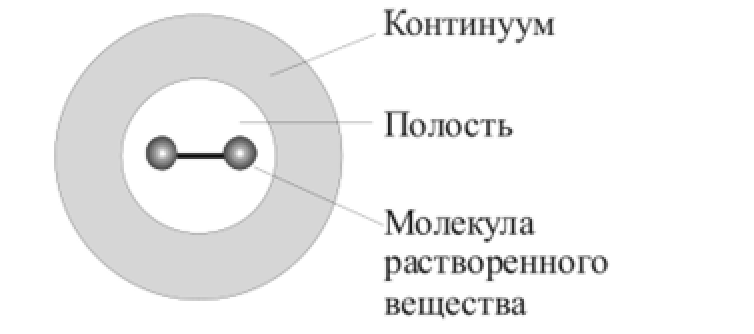
\includegraphics[scale=1.0]{fig/1.jpg}
\caption{Модель поляризуемого континуума}
\end{figure}


\subsubsection{Расчет $pK_a$}
Константа диссоциации кислоты ($K_a$) — константа равновесия реакции диссоциации кислоты на катион водорода и анион кислотного остатка.Чаще вместо самой константы диссоциации $K_a$ используют величину $pK_a$, которая определяется как отрицательный десятичный логарифм самой константы $K_a$:
\mequation{
    pK_a= -\lg \left(K_{a}\right)
}

Величина $pK_a$ связана с разностью энергий между депротонированной и нейтральной формами $D = E^{-} - E^{0}$ следующим теоретическим соотношением (при $T = 293$):
\mequation{
    \left(pK_a\right)_{T}^{'} = \frac{1}{2.3RT}\left(D - \frac{5}{2}RT - 0.41345\right)
}
где 0.41345 Хатри – энергия сольватации протона в водной среде. 

Для получения реального приближенного значения $pK_a$ по полученному значению   используются эмпирические соотношения, зависящие от конкретного варианта метода расчета. В рассматриваемом методе B3LYP/6-31G такое эмпирическое соотношение имеет следующий вид:
\mequation{
    \left(pK_a\right)_{T} = -6.9 + 0.55\left(pK_a\right)_{T}^{'}
}
 	
